% Options for packages loaded elsewhere
\PassOptionsToPackage{unicode}{hyperref}
\PassOptionsToPackage{hyphens}{url}
%
\documentclass[
  8pt,
  ignorenonframetext,
]{beamer}
\usepackage{pgfpages}
\setbeamertemplate{caption}[numbered]
\setbeamertemplate{caption label separator}{: }
\setbeamercolor{caption name}{fg=normal text.fg}
\beamertemplatenavigationsymbolsempty
% Prevent slide breaks in the middle of a paragraph
\widowpenalties 1 10000
\raggedbottom
\setbeamertemplate{part page}{
  \centering
  \begin{beamercolorbox}[sep=16pt,center]{part title}
    \usebeamerfont{part title}\insertpart\par
  \end{beamercolorbox}
}
\setbeamertemplate{section page}{
  \centering
  \begin{beamercolorbox}[sep=12pt,center]{part title}
    \usebeamerfont{section title}\insertsection\par
  \end{beamercolorbox}
}
\setbeamertemplate{subsection page}{
  \centering
  \begin{beamercolorbox}[sep=8pt,center]{part title}
    \usebeamerfont{subsection title}\insertsubsection\par
  \end{beamercolorbox}
}
\AtBeginPart{
  \frame{\partpage}
}
\AtBeginSection{
  \ifbibliography
  \else
    \frame{\sectionpage}
  \fi
}
\AtBeginSubsection{
  \frame{\subsectionpage}
}
\usepackage{amsmath,amssymb}
\usepackage{lmodern}
\usepackage{iftex}
\ifPDFTeX
  \usepackage[T1]{fontenc}
  \usepackage[utf8]{inputenc}
  \usepackage{textcomp} % provide euro and other symbols
\else % if luatex or xetex
  \usepackage{unicode-math}
  \defaultfontfeatures{Scale=MatchLowercase}
  \defaultfontfeatures[\rmfamily]{Ligatures=TeX,Scale=1}
\fi
% Use upquote if available, for straight quotes in verbatim environments
\IfFileExists{upquote.sty}{\usepackage{upquote}}{}
\IfFileExists{microtype.sty}{% use microtype if available
  \usepackage[]{microtype}
  \UseMicrotypeSet[protrusion]{basicmath} % disable protrusion for tt fonts
}{}
\makeatletter
\@ifundefined{KOMAClassName}{% if non-KOMA class
  \IfFileExists{parskip.sty}{%
    \usepackage{parskip}
  }{% else
    \setlength{\parindent}{0pt}
    \setlength{\parskip}{6pt plus 2pt minus 1pt}}
}{% if KOMA class
  \KOMAoptions{parskip=half}}
\makeatother
\usepackage{xcolor}
\newif\ifbibliography
\usepackage{color}
\usepackage{fancyvrb}
\newcommand{\VerbBar}{|}
\newcommand{\VERB}{\Verb[commandchars=\\\{\}]}
\DefineVerbatimEnvironment{Highlighting}{Verbatim}{commandchars=\\\{\}}
% Add ',fontsize=\small' for more characters per line
\usepackage{framed}
\definecolor{shadecolor}{RGB}{248,248,248}
\newenvironment{Shaded}{\begin{snugshade}}{\end{snugshade}}
\newcommand{\AlertTok}[1]{\textcolor[rgb]{0.94,0.16,0.16}{#1}}
\newcommand{\AnnotationTok}[1]{\textcolor[rgb]{0.56,0.35,0.01}{\textbf{\textit{#1}}}}
\newcommand{\AttributeTok}[1]{\textcolor[rgb]{0.77,0.63,0.00}{#1}}
\newcommand{\BaseNTok}[1]{\textcolor[rgb]{0.00,0.00,0.81}{#1}}
\newcommand{\BuiltInTok}[1]{#1}
\newcommand{\CharTok}[1]{\textcolor[rgb]{0.31,0.60,0.02}{#1}}
\newcommand{\CommentTok}[1]{\textcolor[rgb]{0.56,0.35,0.01}{\textit{#1}}}
\newcommand{\CommentVarTok}[1]{\textcolor[rgb]{0.56,0.35,0.01}{\textbf{\textit{#1}}}}
\newcommand{\ConstantTok}[1]{\textcolor[rgb]{0.00,0.00,0.00}{#1}}
\newcommand{\ControlFlowTok}[1]{\textcolor[rgb]{0.13,0.29,0.53}{\textbf{#1}}}
\newcommand{\DataTypeTok}[1]{\textcolor[rgb]{0.13,0.29,0.53}{#1}}
\newcommand{\DecValTok}[1]{\textcolor[rgb]{0.00,0.00,0.81}{#1}}
\newcommand{\DocumentationTok}[1]{\textcolor[rgb]{0.56,0.35,0.01}{\textbf{\textit{#1}}}}
\newcommand{\ErrorTok}[1]{\textcolor[rgb]{0.64,0.00,0.00}{\textbf{#1}}}
\newcommand{\ExtensionTok}[1]{#1}
\newcommand{\FloatTok}[1]{\textcolor[rgb]{0.00,0.00,0.81}{#1}}
\newcommand{\FunctionTok}[1]{\textcolor[rgb]{0.00,0.00,0.00}{#1}}
\newcommand{\ImportTok}[1]{#1}
\newcommand{\InformationTok}[1]{\textcolor[rgb]{0.56,0.35,0.01}{\textbf{\textit{#1}}}}
\newcommand{\KeywordTok}[1]{\textcolor[rgb]{0.13,0.29,0.53}{\textbf{#1}}}
\newcommand{\NormalTok}[1]{#1}
\newcommand{\OperatorTok}[1]{\textcolor[rgb]{0.81,0.36,0.00}{\textbf{#1}}}
\newcommand{\OtherTok}[1]{\textcolor[rgb]{0.56,0.35,0.01}{#1}}
\newcommand{\PreprocessorTok}[1]{\textcolor[rgb]{0.56,0.35,0.01}{\textit{#1}}}
\newcommand{\RegionMarkerTok}[1]{#1}
\newcommand{\SpecialCharTok}[1]{\textcolor[rgb]{0.00,0.00,0.00}{#1}}
\newcommand{\SpecialStringTok}[1]{\textcolor[rgb]{0.31,0.60,0.02}{#1}}
\newcommand{\StringTok}[1]{\textcolor[rgb]{0.31,0.60,0.02}{#1}}
\newcommand{\VariableTok}[1]{\textcolor[rgb]{0.00,0.00,0.00}{#1}}
\newcommand{\VerbatimStringTok}[1]{\textcolor[rgb]{0.31,0.60,0.02}{#1}}
\newcommand{\WarningTok}[1]{\textcolor[rgb]{0.56,0.35,0.01}{\textbf{\textit{#1}}}}
\setlength{\emergencystretch}{3em} % prevent overfull lines
\providecommand{\tightlist}{%
  \setlength{\itemsep}{0pt}\setlength{\parskip}{0pt}}
\setcounter{secnumdepth}{-\maxdimen} % remove section numbering
\newlength{\cslhangindent}
\setlength{\cslhangindent}{1.5em}
\newlength{\csllabelwidth}
\setlength{\csllabelwidth}{3em}
\newlength{\cslentryspacingunit} % times entry-spacing
\setlength{\cslentryspacingunit}{\parskip}
\newenvironment{CSLReferences}[2] % #1 hanging-ident, #2 entry spacing
 {% don't indent paragraphs
  \setlength{\parindent}{0pt}
  % turn on hanging indent if param 1 is 1
  \ifodd #1
  \let\oldpar\par
  \def\par{\hangindent=\cslhangindent\oldpar}
  \fi
  % set entry spacing
  \setlength{\parskip}{#2\cslentryspacingunit}
 }%
 {}
\usepackage{calc}
\newcommand{\CSLBlock}[1]{#1\hfill\break}
\newcommand{\CSLLeftMargin}[1]{\parbox[t]{\csllabelwidth}{#1}}
\newcommand{\CSLRightInline}[1]{\parbox[t]{\linewidth - \csllabelwidth}{#1}\break}
\newcommand{\CSLIndent}[1]{\hspace{\cslhangindent}#1}
% type setting
% ------------------------------------------------------------------------------
\usepackage[german]{babel}     

% fonts
% ------------------------------------------------------------------------------
\usefonttheme{professionalfonts}

% slide title and horizontal line
% ------------------------------------------------------------------------------
\setbeamertemplate{frametitle}{%
    \vskip-30pt \color{black}\large%
    \begin{minipage}[b][23pt]{120mm}%
    \flushleft\insertframetitle%
    \end{minipage}%
}

\setbeamertemplate{headline}										
{
\vskip10pt\hfill\hspace{3.5mm} 										 
\vskip15pt\color{black}\rule{\textwidth}{0.4pt} 					 
}

% slide number
% ---------------------------------------------------------------
\setbeamertemplate{navigation symbols}{}
\setbeamertemplate{footline}
{
\vskip5pt
\vskip2pt
\makebox[123mm]{\hspace{7.5mm}
\hfill Multivariate Datenanalyse $\vert$ 
\copyright $ $ 2023 Dirk Ostwald CC BY-SA 4.0 $\vert$ 
Folie \insertframenumber}
\vskip4pt
}

% block color scheme
% ------------------------------------------------------------------------------
% colors
\definecolor{white}{RGB}{255,255,255}
\definecolor{grey}{RGB}{235,235,235}
\definecolor{lightgrey}{RGB}{245,245,245}
\definecolor{LightBlue}{RGB}{220,220,255}
\definecolor{darkblue}{RGB}{51, 51, 153}

% definitions and theorems
\setbeamercolor{block title}{fg = black, bg = grey}
\setbeamercolor{block body}{fg = black, bg = lightgrey}

% general line spacing 
% ------------------------------------------------------------------------------
\linespread{1.3}

% local line spacing
% ------------------------------------------------------------------------------
\usepackage{setspace}

% colors
% -----------------------------------------------------------------------------
\usepackage{color}

% justified text
% ------------------------------------------------------------------------------
\usepackage{ragged2e}
\usepackage{etoolbox}
\apptocmd{\frame}{}{\justifying}{}

% bullet point lists
% -----------------------------------------------------------------------------
\setbeamertemplate{itemize item}[circle]
\setbeamertemplate{itemize subitem}[circle]
\setbeamertemplate{itemize subsubitem}[circle]
\setbeamercolor{itemize item}{fg = black}
\setbeamercolor{itemize subitem}{fg = black}
\setbeamercolor{itemize subsubitem}{fg = black}
\setbeamercolor{enumerate item}{fg = black}
\setbeamercolor{enumerate subitem}{fg = black}
\setbeamercolor{enumerate subsubitem}{fg = black}
\setbeamerfont{itemize/enumerate body}{}
\setbeamerfont{itemize/enumerate subbody}{size = \normalsize}
\setbeamerfont{itemize/enumerate subsubbody}{size = \normalsize}

% color links
% ------------------------------------------------------------------------------
\usepackage{hyperref}
\definecolor{urls}{RGB}{204,0,0}
\hypersetup{colorlinks, citecolor = darkblue, urlcolor = urls}


% additional math commands
% ------------------------------------------------------------------------------
\usepackage{bm}                               % bold math symbols
\usepackage{mathtools}                        % pmatrix* environment
\newcommand{\niton}{\not\owns}                % reverse not in

% text highlighting
% ------------------------------------------------------------------------------
\usepackage{soul}
\makeatletter
\let\HL\hl
\renewcommand\hl{%
  \let\set@color\beamerorig@set@color
  \let\reset@color\beamerorig@reset@color
  \HL}
\makeatother

% equation highlighting
% -----------------------------------------------------------------------------
\newcommand{\highlight}[2][yellow]{\mathchoice%
  {\colorbox{#1}{$\displaystyle#2$}}%
  {\colorbox{#1}{$\textstyle#2$}}%
  {\colorbox{#1}{$\scriptstyle#2$}}%
  {\colorbox{#1}{$\scriptscriptstyle#2$}}}%

% additional mathematical operators
% ------------------------------------------------------------------------------
\DeclareMathOperator*{\argmax}{arg\,max}
\DeclareMathOperator*{\argmin}{arg\,min}

\ifLuaTeX
  \usepackage{selnolig}  % disable illegal ligatures
\fi
\IfFileExists{bookmark.sty}{\usepackage{bookmark}}{\usepackage{hyperref}}
\IfFileExists{xurl.sty}{\usepackage{xurl}}{} % add URL line breaks if available
\urlstyle{same} % disable monospaced font for URLs
\hypersetup{
  hidelinks,
  pdfcreator={LaTeX via pandoc}}

\author{}
\date{\vspace{-2.5em}}

\begin{document}

\begin{frame}[plain]{}
\protect\hypertarget{section}{}
\center

\begin{center}
\includegraphics[width=0.2\linewidth]{4_Abbildungen/mvda_4_otto} \end{center}

\vspace{2mm}

\Huge

Multivariate Datenanalyse \vspace{6mm}

\large

MSc Psychologie WiSe 2022/23

\vspace{6mm}
\large

Prof.~Dr.~Dirk Ostwald
\end{frame}

\begin{frame}[plain]{}
\protect\hypertarget{section-1}{}
\vfill
\center
\huge

\textcolor{black}{(4) Eigenanalyse} \vfill
\end{frame}

\begin{frame}{}
\protect\hypertarget{section-2}{}
\vfill
\setstretch{3}
\Large

Eigenvektoren und Eigenwerte

Orthonormalzerlegung

Singulärwertzerlegung

Selbstkontrollfragen \vfill 
\end{frame}

\begin{frame}{}
\protect\hypertarget{section-3}{}
\vfill
\setstretch{3}
\Large

\textbf{Eigenvektoren und Eigenwerte}

Orthonormalzerlegung

Singulärwertzerlegung

Selbstkontrollfragen \vfill 
\end{frame}

\begin{frame}{Eigenvektoren und Eigenwerte}
\protect\hypertarget{eigenvektoren-und-eigenwerte}{}
\small
\begin{definition}[Eigenvektor, Eigenwert]
$A \in \mathbb{R}^{m \times m}$ sei eine quadratische Matrix. Dann heißt jeder
Vektor $v \in \mathbb{R}^m, v \neq 0_m$, für den gilt, dass
\begin{equation}
Av  = \lambda v
\end{equation}
mit $\lambda \in \mathbb{R}$ ein \textit{Eigenvektor} von $A$. $\lambda$
heißt zugehöriger \textit{Eigenwert} von $A$.
\end{definition}
\footnotesize

Bemerkungen

\begin{itemize}
\tightlist
\item
  Ein Eigenvektor \(v\) von \(A\) wird durch \(A\) mit einem Faktor
  \(\lambda\) verlängert.
\item
  Jeder Eigenvektor hat einen zugehörigen Eigenwert.
\item
  Die Eigenwerte verschiedener Eigenvektor können identisch sein.
\end{itemize}
\end{frame}

\begin{frame}{Eigenvektoren und Eigenwerte}
\protect\hypertarget{eigenvektoren-und-eigenwerte-1}{}
\small
\begin{theorem}[Multiplikativität von Eigenvektoren]
\justifying
\normalfont
$A \in \mathbb{R}^{m \times m}$ sei eine quadratische Matrix. Wenn $v \in \mathbb{R}^m$
Eigenvektor von $A$ mit Eigenwert $\lambda \in \mathbb{R}$ ist, dann ist für $c \in \mathbb{R}$ 
auch $cv \in \mathbb{R}^m $ Eigenvektor von $A$ und zwar wiederum mit Eigenwert $\lambda \in \mathbb{R}$.
\end{theorem}

\footnotesize

\underline{Beweis}

Es gilt \begin{equation}
Av = \lambda v   \Leftrightarrow 
cAv = c\lambda v \Leftrightarrow 
A(cv) = \lambda(cv)
\end{equation} Also ist \(cv\) ein Eigenvektor von \(A\) mit Eigenwert
\(\lambda\).

\(\hfill\Box\)

\normalsize

\textbf{Konvention}

Wir betrachten im Folgenden nur Eigenvektoren mit \(\Vert v \Vert = 1\).
\end{frame}

\begin{frame}[t]{Eigenvektoren und Eigenwerte}
\protect\hypertarget{eigenvektoren-und-eigenwerte-2}{}
\vspace{2mm}

\textcolor{darkblue}{Visualisierung eines Eigenvektors} \footnotesize
\vspace{2mm}

Für \(A := \begin{pmatrix} 2 & 1 \\ 1 & 2 \end{pmatrix}\) ist
\(v := \frac{1}{\sqrt{2}} \begin{pmatrix} 1 \\ 1 \end{pmatrix}\)
Eigenvektor zum Eigenwert
\(\lambda = 3, w := \begin{pmatrix} 1 \\ 0 \end{pmatrix}\) ist kein
Eigenvektor.

\center

\begin{center}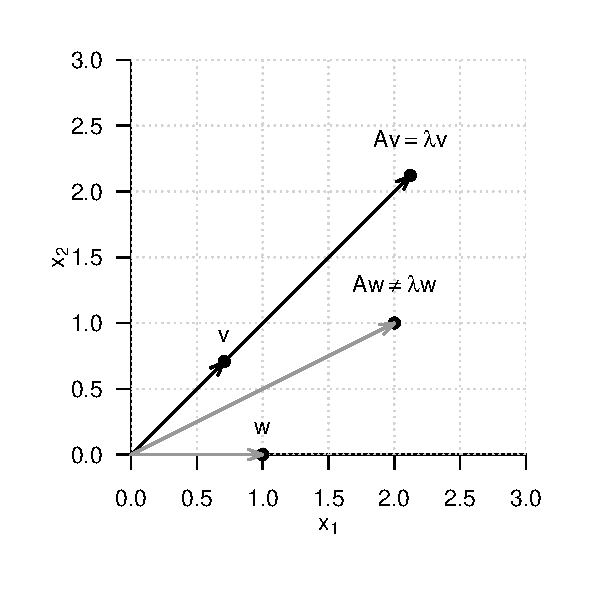
\includegraphics[width=0.55\linewidth]{4_Abbildungen/mvda_4_eigenvektor} \end{center}
\end{frame}

\begin{frame}[fragile]{Eigenvektoren und Eigenwerte}
\protect\hypertarget{eigenvektoren-und-eigenwerte-3}{}
\small
\begin{theorem}[Bestimmung von Eigenwerten und Eigenvektoren]
\normalfont
\justifying
$A \in \mathbb{R}^{m \times m}$ sei eine quadratische Matrix. Dann ergeben sich
die Eigenwerte von $A$ als die Nullstellen des \textit{charakteristischen Polynoms}
\begin{equation}
\chi_A(\lambda) := \det(A - \lambda I_m) 
\end{equation}
von $A$. Weiterhin seien $\lambda_i^*, i = 1,2,...$ die auf diese Weise bestimmten
Eigenwerte von $A$. Die entsprechenden Eigenvektoren $v_i, i = 1,2,...$ von $A$
können dann durch Lösen der linearen Gleichungssysteme
\begin{equation}
(A - \lambda_i^* I_m)v_i = 0_m \mbox{ für } i = 1,2,...
\end{equation}
bestimmt werden.
\end{theorem}

\footnotesize

Bemerkungen

\begin{itemize}
\tightlist
\item
  Für kleine Matrizen mit \(m \le 3\) können Eigenwerte und
  Eigenvektoren manuell bestimmt werden.
\item
  Bei großen Matrizen werden Eigenwerte und Eigenvektor im Allgemeinen
  numerisch bestimmt.
\item
  R's \texttt{eigen()}, Scipy's \texttt{linalg.eig()}, Matlab's
  \texttt{eig()}.
\end{itemize}
\end{frame}

\begin{frame}{Eigenvektoren und Eigenwerte}
\protect\hypertarget{eigenvektoren-und-eigenwerte-4}{}
\setstretch{1.2}
\footnotesize

\underline{Beweis}

\noindent (1) Bestimmen von Eigenwerten

Wir halten zunächst fest, dass mit der Definition von Eigenvektoren und
Eigenwerten gilt, dass \begin{equation}
Av = \lambda v
\Leftrightarrow Av - \lambda v = 0_m
\Leftrightarrow (A - \lambda I_m)v = 0_m.
\end{equation} Für den Eigenwert \(\lambda\) wird der Eigenvektor \(v\)
also durch \((A - \lambda I_m)\) auf den Nullvektor \(0_m\) abgebildet.
Weil aber per Definition \(v \neq 0_m\) gilt, ist die Matrix
\((A - \lambda I_m)\) somit nicht invertierbar: sowohl der Nullvektor
als auch \(v\) werden durch \(A\) auf \(0_m\) abgebildet, die Abbildung
\begin{equation}
f : \mathbb{R}^m \to \mathbb{R}^m, x \mapsto (A - \lambda I_m)x
\end{equation} ist also nicht bijektiv, und \((A - \lambda I_m)^{-1}\)
kann nicht existieren. Die Tatsache, dass \((A - \lambda I_m)\) nicht
invertierbar ist, ist aber äquivalent dazu, dass die Determinante von
\((A -\lambda I_m)\) Null ist. Also ist \begin{equation}
\chi_A(\lambda) = \det(A - \lambda I_m) = 0
\end{equation} notwendige und hinreichende Bedingung dafür, dass
\(\lambda\) ein Eigenwert von \(A\) ist.

\noindent (2) Bestimmen von Eigenvektoren

Es sei \(\lambda_i^*\) ein Eigenwert von \(A\). Dann gilt mit den obigen
Überlegungen, dass Auflösen von \begin{equation}
(A - \lambda_i^* I_m)v_i^* = 0_m
\end{equation} nach \(v_i^*\) einen Eigenvektor zum Eigenwert
\(\lambda^*\) ergibt.

\(\hfill \Box\)
\end{frame}

\begin{frame}{Eigenvektoren und Eigenwerte}
\protect\hypertarget{eigenvektoren-und-eigenwerte-5}{}
\setstretch{1.6}

Beispiel

\footnotesize

Es sei \begin{equation}
A :=
\begin{pmatrix*}[r]
2 & 1 \\
1 & 2\end{pmatrix*}
\end{equation} Wir wollen die Eigenwerte und Eigenvektoren von \(A\)
bestimmen. \vspace{1mm}

\small

\noindent (1) Berechnen von Eigenwerten \footnotesize

Die Eigenwerte von \(A\) sind die Nullstellen des charakteristischen
Polynoms von \(A\).

Das charakteristische Polynom von \(A\) ergibt als \begin{equation}
\chi_A(\lambda)
=
\det\left(
\begin{pmatrix*}[r]
2 & 1 \\
1 & 2\end{pmatrix*}
-
\begin{pmatrix*}[r]
\lambda & 0 \\
0       & \lambda
\end{pmatrix*}
\right)
=
\det
\begin{pmatrix*}[r]
2 - \lambda & 1 \\
1 & 2 - \lambda
\end{pmatrix*}
= (2 - \lambda)^2 - 1.
\end{equation} Nullsetzen und Auflösen nach \(\lambda\) ergibt mit der
\href{https://de.wikipedia.org/wiki/Quadratische_Gleichung}{\textcolor{blue}{pq-Formel}}
\begin{equation}
(2 - \lambda)^2 - 1 = 0 \Rightarrow \lambda_1 = 3, \lambda_2 = 1.
\end{equation} Die Eigenwerte von \(A\) sind also \(\lambda_1 = 3\) und
\(\lambda_2 = 1\).
\end{frame}

\begin{frame}{Eigenvektoren und Eigenwerte}
\protect\hypertarget{eigenvektoren-und-eigenwerte-6}{}
\setstretch{1.6}

Beispiel (fortgeführt)

\small

\noindent (2) Berechnen von Eigenvektoren

\footnotesize

Die Eigenvektoren zu den Eigenwerten \(\lambda_1 = 3\) und
\(\lambda_2 = 1\) ergeben sich durch Lösen der linearen
Gleichungssysteme \begin{equation}
(A - \lambda_i I_2)v_i = 0_2 \mbox{ für } i = 1,2.
\end{equation} Für \(\lambda_1 = 3\) ergibt sich \begin{equation}
(A - 3I_2)v_1 = 0_2
\Leftrightarrow
\begin{pmatrix*}[r]
-1 & 1 \\
 1 & -1
\end{pmatrix*}
\begin{pmatrix*}[r]
v_{1_1} \\
v_{1_2}
\end{pmatrix*}
=
\begin{pmatrix*}[r]
0 \\
0
\end{pmatrix*}
\Rightarrow
v_1 =
\frac{1}{\sqrt{2}}
\begin{pmatrix*}[r]
1 \\
1
\end{pmatrix*}
\mbox{ ist eine Lösung. }
\end{equation} Fpr \(\lambda_2 = 1\) ergibt sich \begin{equation}
(A - 1I_2)v_2 = 0_2
\Leftrightarrow
\begin{pmatrix*}[r]
1 & 1 \\
1 & 1
\end{pmatrix*}
\begin{pmatrix*}[r]
v_{2_1} \\
v_{2_2}
\end{pmatrix*}
=
\begin{pmatrix*}[r]
0 \\
0
\end{pmatrix*}
\Rightarrow
v_2 =
\frac{1}{\sqrt{2}}
\begin{pmatrix*}[r]
-1 \\
 1
\end{pmatrix*}
\mbox{ ist eine Lösung. }
\end{equation} Weiterhin gilt \(v_1^Tv_2 = 0\) und
\(||v_1|| = ||v_2|| = 1\).
\end{frame}

\begin{frame}[fragile]{Eigenvektoren und Eigenwerte}
\protect\hypertarget{eigenvektoren-und-eigenwerte-7}{}
Beispiel (fortgeführt) \vspace{3mm} \footnotesize

\begin{Shaded}
\begin{Highlighting}[]
\CommentTok{\# Matrixdefinition}
\NormalTok{A }\OtherTok{=} \FunctionTok{matrix}\NormalTok{(}\FunctionTok{c}\NormalTok{(}\DecValTok{2}\NormalTok{,}\DecValTok{1}\NormalTok{,}
             \DecValTok{1}\NormalTok{,}\DecValTok{2}\NormalTok{),}
           \AttributeTok{nrow  =} \DecValTok{2}\NormalTok{,}
           \AttributeTok{byrow =} \ConstantTok{TRUE}\NormalTok{)}

\CommentTok{\# Eigenanalyse}
\FunctionTok{eigen}\NormalTok{(A)}
\end{Highlighting}
\end{Shaded}

\begin{verbatim}
> eigen() decomposition
> $values
> [1] 3 1
> 
> $vectors
>       [,1]   [,2]
> [1,] 0.707 -0.707
> [2,] 0.707  0.707
\end{verbatim}
\end{frame}

\begin{frame}{}
\protect\hypertarget{section-4}{}
\vfill
\setstretch{3}
\Large

Eigenvektoren und Eigenwerte

\textbf{Orthonormalzerlegung}

Singulärwertzerlegung

Selbstkontrollfragen \vfill 
\end{frame}

\begin{frame}{Orthonormalzerlegung}
\protect\hypertarget{orthonormalzerlegung}{}
\small
\begin{theorem}[Eigenwerte und Eigenvektoren symmetrischer Matrizen]
\justifying
\normalfont
$S \in \mathbb{R}^{m \times m}$ sei eine symmetrische Matrix. Dann gelten
\begin{itemize}
\item[(1)] Die Eigenwerte von $S$ sind reell.
\item[(2)] Die Eigenvektoren zu je zwei verschiedenen Eigenwerten von $S$ sind orthogonal. 
\end{itemize}
\end{theorem}
\footnotesize

Bemerkung

\begin{itemize}
\tightlist
\item
  \justifying In nachfolgendem Beweis setzen wir die Tatsache dass eine
  symmetrische \(m\) reelle Eigenwerte hat als gegeben voraus und zeigen
  lediglich, dass die Eigenvektoren zu je zwei verschiedenen Eigenwerten
  einer symmetrischen Matrix orthogonal sind. Ein vollständiger Beweis
  des Theorems findet sich in Strang (2009), Kapitel 6.4.
\item
  Da wir als Eigenvektoren nur Eigenvektoren der Länge 1 betrachten,
  sind die hier angesprochenen orthogonalen Eigenvektoren insbesondere
  auch orthonormal.
\end{itemize}
\end{frame}

\begin{frame}{Orthonormalzerlegung}
\protect\hypertarget{orthonormalzerlegung-1}{}
\footnotesize

\underline{Beweis}

Ohne Beschränkung der Allgemeinheit seien \(\lambda_i\) und
\(\lambda_j\) mit \(1 \le i,j \le m\) und \(\lambda_i \neq \lambda_j\)
zwei verschiedenen Eigenwerte von \(S\) mit zugehörigen Eigenvektoren
\(q_i\) und \(q_j\), respektive. Dann ergibt sich wie unten gezeigt,
dass \begin{equation}
\lambda_i q_i^Tq_j = \lambda_j q_i^Tq_j.
\end{equation} Mit \(q_i \neq 0_m, q_j \neq 0_m\) und
\(\lambda_i \neq \lambda_j\) folgt damit \(q_i^Tq_j = 0\), weil weil es
keine andere Zahl \(c\) als die Null gibt, für die bei
\(a,b\in \mathbb{R}\) und \(a \neq b\) gilt, dass \begin{equation}
ac = bc.
\end{equation} Um \begin{equation}
\lambda_i q_i^Tq_j = \lambda_j q_i^Tq_j.
\end{equation} zu zeigen, halten wir zunächst fest, dass
\begin{equation}
                 Sq_i       = \lambda_i q_i      
\Leftrightarrow (Sq_i)^T    = (\lambda_i q_i)^T  
\Leftrightarrow q_i^TS^T    = q_i^T \lambda_i^T  
\Leftrightarrow q_i^T S     = q_i^T \lambda_i   
\Leftrightarrow q_i^T Sq_j  = \lambda_i q_i^Tq_j 
\end{equation} und \begin{equation}
                     Sq_j = \lambda_j q_j
\Leftrightarrow q_i^TSq_j = \lambda_j q_i^Tq_j
\end{equation} gelten. Sowohl \(\lambda_i q_i^Tq_j\) als auch
\(\lambda_j q_i^Tq_j\) sind also mit \(q_i^T Sq_j\) und damit auch
miteinander identisch.

\(\hfill \Box\)
\end{frame}

\begin{frame}{Orthonormalzerlegung}
\protect\hypertarget{orthonormalzerlegung-2}{}
\setstretch{1.2}
\footnotesize
\begin{theorem}[Orthonormale Zerlegung einer symmetrischen Matrix]
\normalfont
$S \in \mathbb{R}^{m \times m}$ sei eine symmetrische Matrix mit $m$ verschiedenen
Eigenwerten. Dann kannn $S$
geschrieben werden als
\begin{equation}
S = Q \Lambda Q^T,
\end{equation}
wobei $Q \in \mathbb{R}^{m \times m}$ eine orthogonale Matrix ist und
$\Lambda \in \mathbb{R}^{m\times m}$ eine Diagonalmatrix ist.
\end{theorem}
\vspace{-1mm}

Bemerkungen \vspace{-1mm}

\begin{itemize}
\tightlist
\item
  \(S = Q \Lambda Q^T\) heißt auch \emph{Diagonalisierung} von \(S\).
\item
  Wie im Beweis gezeigt wählt man als Spalten von \(Q\) die
  orthonormalen Eigenvektoren von \(S\).
\item
  Wie im Beweis gezeigt wählt man als Diagonalelemente von \(\Lambda\)
  die zugehörigen Eigenwerte von \(S\).
\end{itemize}

\footnotesize

\underline{Beweis}

Es seien \(\lambda_1,...,\lambda_m\) die Eigenwerte von \(S\) und
\(q_1,...,q_m\) die zugehörigen orthonormalen Eigenvektoren. Mit
\begin{equation}
Q :=
\begin{pmatrix*}[r]
q_1 & q_2 & \cdots & q_m
\end{pmatrix*}
\in \mathbb{R}^{m \times m}
\mbox{ und }
\Lambda :=
\mbox{diag}\begin{pmatrix*}[r]
\lambda_1,\lambda_2,...,\lambda_m
\end{pmatrix*}
\in \mathbb{R}^{m \times m},
\end{equation} folgt dann mit den Definitionen von Eigenwerten und
Eigenvektoren, dass \begin{equation}
Sq_i = \lambda_i q_i \mbox{ für } i = 1,...,m
\Leftrightarrow
Sq_i = q_i \lambda_i \mbox{ für } i = 1,...,m
\Leftrightarrow
SQ = Q\Lambda.
\end{equation} Rechtseitige Multiplikation mit \(Q^T\) ergibt dann mit
\(QQ^T = I_m\), dass \begin{equation}
SQQ^T = Q \Lambda Q^T
\Leftrightarrow SI_m = Q \Lambda Q^T
\Leftrightarrow S    = Q \Lambda Q^T.
\end{equation} \(\hfill \Box\)
\end{frame}

\begin{frame}{Orthonormalzerlegung}
\protect\hypertarget{orthonormalzerlegung-3}{}
\setstretch{1.12}
\small
\vspace{2mm}

Beispiel (fortgeführt)

\footnotesize

Für die symmetrische Matrix \begin{equation}
A = \begin{pmatrix} 2 & 1 \\ 1 & 2 \end{pmatrix}
\end{equation} mit den oben bestimmten Eigenwerten
\(\lambda_1 = 3,\lambda_2 = 1\) und zugehörigen orthonormalen
Eigenvektoren \begin{equation}
v_1 = \frac{1}{\sqrt{2}}
\begin{pmatrix*}[r]
1 \\
1 
\end{pmatrix*},
v_2 = \frac{1}{\sqrt{2}}
\begin{pmatrix*}[r]
-1 \\
1 
\end{pmatrix*}
\end{equation} seien \begin{equation}
Q := \begin{pmatrix*}[r]
v_1 & v_2
\end{pmatrix*}
\mbox{ und }
\Lambda = \mbox{diag}(\lambda_1,\lambda_2).
\end{equation} Dann ergibt sich \begin{align*}
Q\Lambda Q^T
& =
\begin{pmatrix*}[r]
v_1 & v_2
\end{pmatrix*}
\mbox{diag}(\lambda_1,\lambda_2)
\begin{pmatrix*}[r]
v_1 & v_2
\end{pmatrix*}^T \\
& =
\left(
\frac{1}{\sqrt{2}}
\begin{pmatrix*}[r]
1 & -1\\
1 &  1
\end{pmatrix*}
\begin{pmatrix*}[r]
3 & 0 \\
0 & 1
\end{pmatrix*}
\right)
\left(
\frac{1}{\sqrt{2}}
\begin{pmatrix*}[r]
 1 &  1 \\
-1 &  1
\end{pmatrix*}
\right)
\\
& =
\left(
\frac{1}{\sqrt{2}}
\begin{pmatrix*}[r]
3 & -1 \\
3 &  1
\end{pmatrix*}
\right)
\left(
\frac{1}{\sqrt{2}}
\begin{pmatrix*}[r]
 1 &  1 \\
-1 &  1
\end{pmatrix*}
\right)
\\
& =
\frac{1}{2}
\begin{pmatrix*}[r]
4 & 2 \\
2 & 4
\end{pmatrix*} \\
& =
\begin{pmatrix*}[r]
2 & 1 \\
1 & 2
\end{pmatrix*} \\
& = A.
\end{align*}
\end{frame}

\begin{frame}{}
\protect\hypertarget{section-5}{}
\vfill
\setstretch{3}
\Large

Eigenvektoren und Eigenwerte

Orthonormalzerlegung

\textbf{Singulärwertzerlegung}

Selbstkontrollfragen \vfill 
\end{frame}

\begin{frame}[fragile]{Singulärwertzerlegung}
\protect\hypertarget{singuluxe4rwertzerlegung}{}
\small
\begin{definition}[Singulärwertzerlegung]
\justifying
$Y \in \mathbb{R}^{m \times n}$ sei eine Matrix. Dann heißt die Zerlegung
\begin{equation}
Y = USV^T,
\end{equation}
wobei $U \in \mathbb{R}^{m \times m}$ eine orthogonale Matrix ist, $S \in \mathbb{R}^{m \times n}$
eine Diagonalmatrix ist und $V \in \mathbb{R}^{n \times n}$ eine orthogonale Matrix ist,
\textit{Singulärwertzerlegung (Singular Value Decomposition (SVD))} von $Y$. Die
Diagonalelemente von  $S$ heißen die  \textit{Singulärwerte} von $Y$.
\end{definition}

\footnotesize

Bemerkungen

\begin{itemize}
\tightlist
\item
  Für eine ausführliche Diskussion der Singulärwertzerlegung siehe z.B.
  Strang (2009), Kapitel 7.
\item
  Singulärwertzerlegungen können in R mit \texttt{svd()} berechnet
  werden.
\end{itemize}
\end{frame}

\begin{frame}{Singulärwertzerlegung}
\protect\hypertarget{singuluxe4rwertzerlegung-1}{}
\small
\begin{theorem}[Singulärwertzerlegung und Eigenanalyse]
\justifying
\normalfont
$Y \in \mathbb{R}^{m \times n}$ sei eine Matrix und
\begin{equation}
Y = USV^T
\end{equation}
sei ihre Singulärwertzerlegung. Dann gilt:
\begin{itemize}
\item Die Spalten von $U$ sind die Eigenvektoren von $YY^T$,
\item die Spalten von $V$ sind die Eigenvektoren von $Y^TY$ und
\item die entsprechenden Singulärwerte sind die Quadratwurzeln der zugehörigen Eigenwerte.
\end{itemize}
\end{theorem}
\footnotesize

Bemerkung

\begin{itemize}
\tightlist
\item
  Singulärwertzerlegung und Eigenanalyse sind eng verwandt.
\end{itemize}
\end{frame}

\begin{frame}{Singulärwertzerlegung}
\protect\hypertarget{singuluxe4rwertzerlegung-2}{}
\footnotesize

\underline{Beweis} \vspace{1mm}

Wir halten zunächst fest, dass mit \begin{equation}
\left(YY^T\right)^T = YY^T \mbox{ und } \left(Y^TY\right)^T = Y^TY,
\end{equation} \(YY^T\) und \(Y^TY\) symmetrische Matrizen sind und
somit Orthornomalzerlegungen haben. Wir halten weiterhin fest, dass mit
\(V^TV = I_n\), \(U^TU = I_m\) und \(S^T = S\) gilt, dass
\begin{equation}
YY^T
= USV^T \left(USV^T\right)^T
= USV^TVS^TU^T
= USSU^T
=: U\Lambda U^T
\end{equation} und \begin{equation}
Y^TY
= \left(USV^T\right)^T USV^T
= VS^TU^T US^T V^T
=: V\Lambda V^T
\end{equation} ist, wobei wir \(\Lambda := SS\) definiert haben. Weil
das Produkt von Diagonalmatrizen wieder eine Diagonalmatrix ist, ist
\(\Lambda\) eine Diagonalmatrix und per Definition sind \(U\) und \(V\)
orthogonale Matrizen. Wir haben also \(YY^T\) und \(Y^TY\) in Form der
Orthonormalzerlegungen \begin{equation}
YY^T = U \Lambda U^T  \mbox{ und } Y^TY = V \Lambda V^T
\end{equation} geschrieben, wobei für die Diagonalelemente von
\(\Lambda\) gilt, dass sie die quadrierten Werte der Diagonalemente von
\(S\) sind.

\(\hfill \Box\)
\end{frame}

\begin{frame}{}
\protect\hypertarget{section-6}{}
\vfill
\setstretch{3}
\Large

Eigenvektoren und Eigenwerte

Orthonormalzerlegung

Singulärwertzerlegung

\textbf{Selbstkontrollfragen} \vfill 
\end{frame}

\begin{frame}{Selbstkontrollfragen}
\protect\hypertarget{selbstkontrollfragen}{}
\footnotesize
\setstretch{3}
\begin{enumerate}
\item Geben Sie die Definition eines Eigenvektors und eines Eigenwertes einer quadratischen Matrix wieder.
\item Geben Sie das Theorem zur Bestimmung von Eigenwerten und Eigenvektoren wieder.
\item Geben Sie das Theorem zu den Eigenwerten und Eigenvektoren symmetrischer Matrizen wieder.
\item Geben Sie das Theorem zur orthonormalen Zerlegung einer symmetrischen Matrix wieder.
\item Geben Sie die Definition einer Singulärwertzerlegung wieder.
\item Geben Sie das Theorem zum Zusammenhang von Singulärwertzerlegung und Eigenanalyse wieder.
\end{enumerate}
\end{frame}

\begin{frame}{References}
\protect\hypertarget{references}{}
\footnotesize

\hypertarget{refs}{}
\begin{CSLReferences}{1}{0}
\leavevmode\vadjust pre{\hypertarget{ref-strang_2009}{}}%
Strang, Gilbert. 2009. \emph{Introduction to {Linear Algebra}}.

\end{CSLReferences}
\end{frame}

\end{document}
